\newpage
\subsection{Caso d'uso UC7: Visualizzazione API}
\label{UC7}
\begin{figure}[ht]
	\centering
	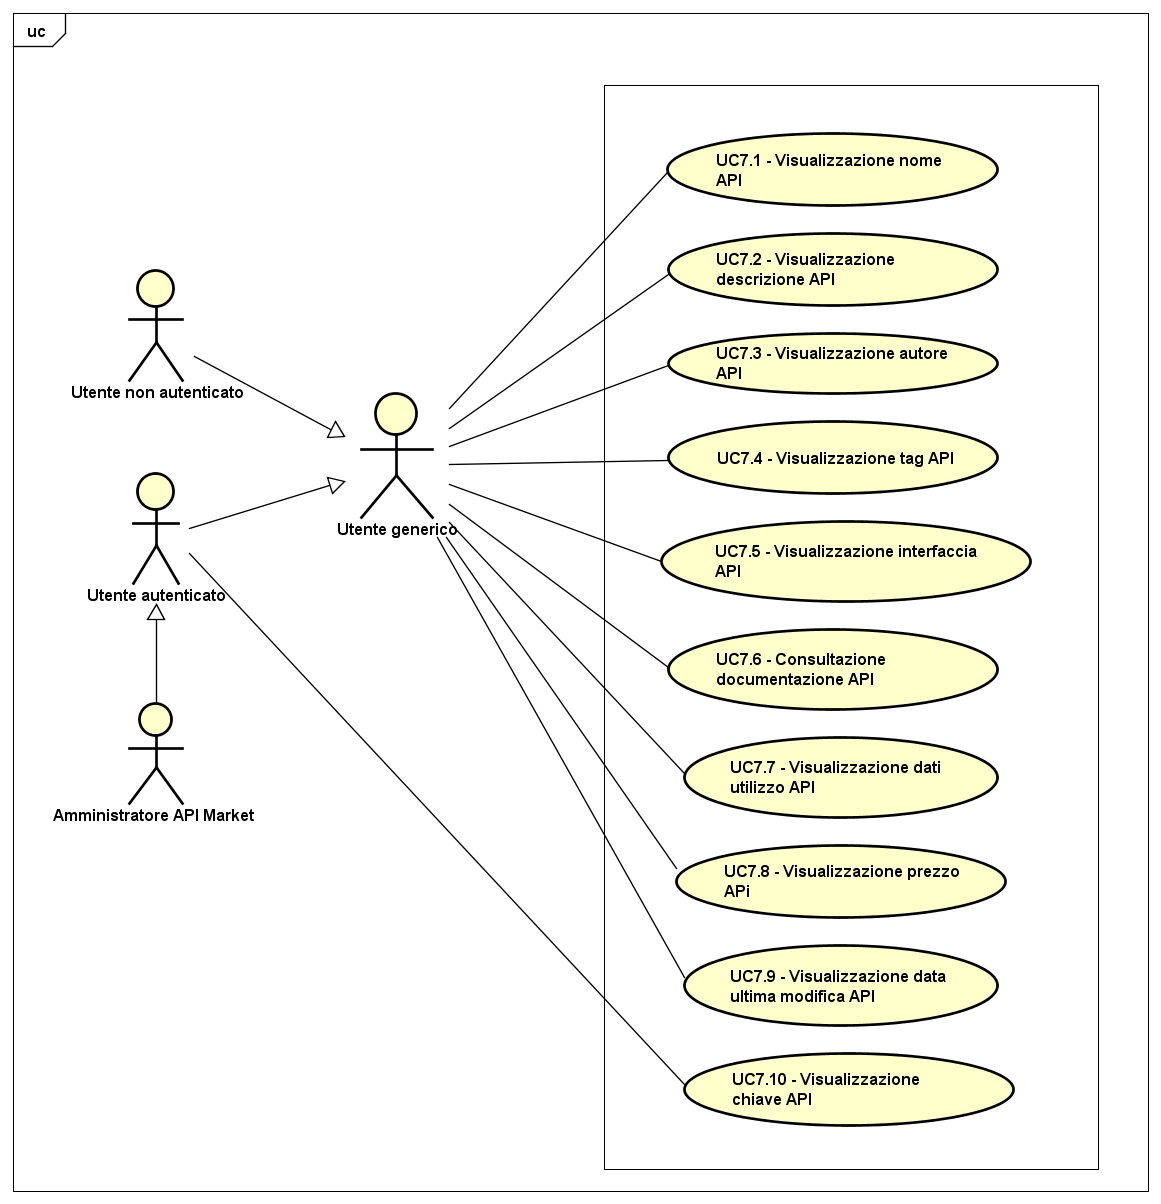
\includegraphics[scale=0.45]{UML/UC7.png}
	\caption{UC7: Visualizzazione API}
\end{figure}

\begin{longtable}{ l | p{11cm}}
	\hline
	\rowcolor{Gray}
	\multicolumn{2}{c}{UC7 - Visualizzazione API}\\
	\hline
	
	 \textbf{Attori} & Utente generico \\
	\textbf{Descrizione} & L'attore visualizza i dati relativi ad una API \\
	\textbf{Pre-Condizioni} & L'attore ha selezionato una API tramite un link (E.g: Ottenuto da una ricerca) \\
	\textbf{Post-Condizioni} & L'attore ha visualizzato i dati relativi all'API selezionata \\
	\textbf{Scenario Principale} &
	\begin{enumerate*}[label=(\arabic*.),itemjoin={\newline}]
		\item L'attore può visualizzare il nome dell'API (UC7.1)
		\item L'attore può visualizzare la descrizione dell'API (UC7.2)
		\item L'attore può visualizzare il nome dell'autore dell'API (UC7.3)
		\item L'attore può visualizzare la categoria dell'API (UC7.4)
		\item L'attore può visualizzare l'interfaccia dell'API (UC7.5)
		\item L'attore può consultare la documentazione dell'API (UC7.6)
		\item L'attore può visualizzare i dati di utilizzo dell'API (UC7.7)
		\item L'attore può visualizzare il prezzo dell'API (UC7.8)
		\item L'attore può visualizzare la data dell'ultima modifica all'API (UC7.9)
		\item L'attore può visualizzare la versione dell'API (UC7.10)
		\item L'attore può visualizzare il logo dell'API (UC7.11)
		\item L'attore può visualizzare la policy di vendita dell'API (UC7.12)
		\item L'attore può visualizzare il link alla pagine d'acquisto dell'API (UC7.13)
	\end{enumerate*}\\
\end{longtable}


\subsubsection{Caso d'uso UC7.1: Visualizzazione nome API}
\label{UC7_1}

\begin{minipage}{\linewidth}
	\begin{tabular}{ l | p{11cm}}
		\hline
		\rowcolor{Gray}
		\multicolumn{2}{c}{UC7.1 - Visualizzazione nome API} \\
		\hline
		\textbf{Attori} & Utente generico \\
		\textbf{Descrizione} & L'attore visualizza nella schermata relativa il nome dell'API \\
		\textbf{Pre-Condizioni} & L'attore si trova nella schermata di visualizzazione API dell'API precedentemente selezionata \\
		\textbf{Post-Condizioni} & L'attore ha visualizzato il nome dell'API selezionata \\
		\textbf{Scenario Principale} & 
		\begin{enumerate*}[label=(\arabic*.),itemjoin={\newline}]
			\item L'attore può visualizzare il nome dell'API selezionata
		\end{enumerate*}\\
	\end{tabular}
\end{minipage}

\subsubsection{Caso d'uso UC7.2: Visualizzazione descrizione API}
\label{UC7_2}

\begin{minipage}{\linewidth}
	\begin{tabular}{ l | p{11cm}}
		\hline
		\rowcolor{Gray}
		\multicolumn{2}{c}{UC7.2 - Visualizzazione descrizione API} \\
		\hline
		\textbf{Attori} & Utente generico \\
		\textbf{Descrizione} & L'attore visualizza nella schermata relativa la descrizione dell'API \\
		\textbf{Pre-Condizioni} & L'attore si trova nella schermata di visualizzazione API dell'API precedentemente selezionata \\
		\textbf{Post-Condizioni} & L'attore ha visualizzato la descrizione dell'API selezionata \\
		\textbf{Scenario Principale} & 
		\begin{enumerate*}[label=(\arabic*.),itemjoin={\newline}]
			\item L'attore può visualizzare la descrizione dell'API selezionata
		\end{enumerate*}\\
	\end{tabular}
\end{minipage}

\subsubsection{Caso d'uso UC7.3: Visualizzazione autore API}
\label{UC7_3}

\begin{minipage}{\linewidth}
	\begin{tabular}{ l | p{11cm}}
		\hline
		\rowcolor{Gray}
		\multicolumn{2}{c}{UC7.3 - Visualizzazione autore API} \\
		\hline
		\textbf{Attori} & Utente generico \\
		\textbf{Descrizione} & L'attore visualizza nella schermata relativa il nome dell'autore dell'API \\
		\textbf{Pre-Condizioni} & L'attore si trova nella schermata di visualizzazione API dell'API precedentemente selezionata \\
		\textbf{Post-Condizioni} & L'attore ha visualizzato il nome dell'autore per l'API selezionata \\
		\textbf{Scenario Principale} & 
		\begin{enumerate*}[label=(\arabic*.),itemjoin={\newline}]
			\item L'attore può visualizzare il nome dell'autore per l'API selezionata
		\end{enumerate*}\\
	\end{tabular}
\end{minipage}

\subsubsection{Caso d'uso UC7.4: Visualizzazione categoria API}
\label{UC7_4}

\begin{minipage}{\linewidth}
	\begin{tabular}{ l | p{11cm}}
		\hline
		\rowcolor{Gray}
		\multicolumn{2}{c}{UC7.4 - Visualizzazione tag API} \\
		\hline
		\textbf{Attori} & Utente generico \\
		\textbf{Descrizione} & L'attore visualizza nella schermata relativa la categoria dell'API \\
		\textbf{Pre-Condizioni} & L'attore si trova nella schermata di visualizzazione API dell'API precedentemente selezionata \\
		\textbf{Post-Condizioni} & L'attore ha visualizzato la categoria dell'API selezionata \\
		\textbf{Scenario Principale} & 
		\begin{enumerate*}[label=(\arabic*.),itemjoin={\newline}]
			\item L'attore può visualizzare la categoria dell'API selezionata
		\end{enumerate*}\\
	\end{tabular}
\end{minipage}

\subsubsection{Caso d'uso UC7.5: Visualizzazione interfaccia API}
\label{UC7_5}

\begin{minipage}{\linewidth}
	\begin{tabular}{ l | p{11cm}}
		\hline
		\rowcolor{Gray}
		\multicolumn{2}{c}{UC7.5 - Visualizzazione interfaccia API} \\
		\hline
		\textbf{Attori} & Utente generico \\
		\textbf{Descrizione} & L'attore visualizza nella schermata relativa l'interfaccia dell'API \\
		\textbf{Pre-Condizioni} & L'attore si trova nella schermata di visualizzazione API dell'API precedentemente selezionata \\
		\textbf{Post-Condizioni} & L'attore ha visualizzato l'interfaccia dell'API selezionata \\
		\textbf{Scenario Principale} & 
		\begin{enumerate*}[label=(\arabic*.),itemjoin={\newline}]
			\item L'attore può visualizzare l'interfaccia dell'API selezionata
		\end{enumerate*}\\
	\end{tabular}
\end{minipage}

\newpage
\subsubsection{Caso d'uso UC7.6: Consultazione documentazione API}
\label{UC7_6}
\begin{figure}[ht]
	\centering
	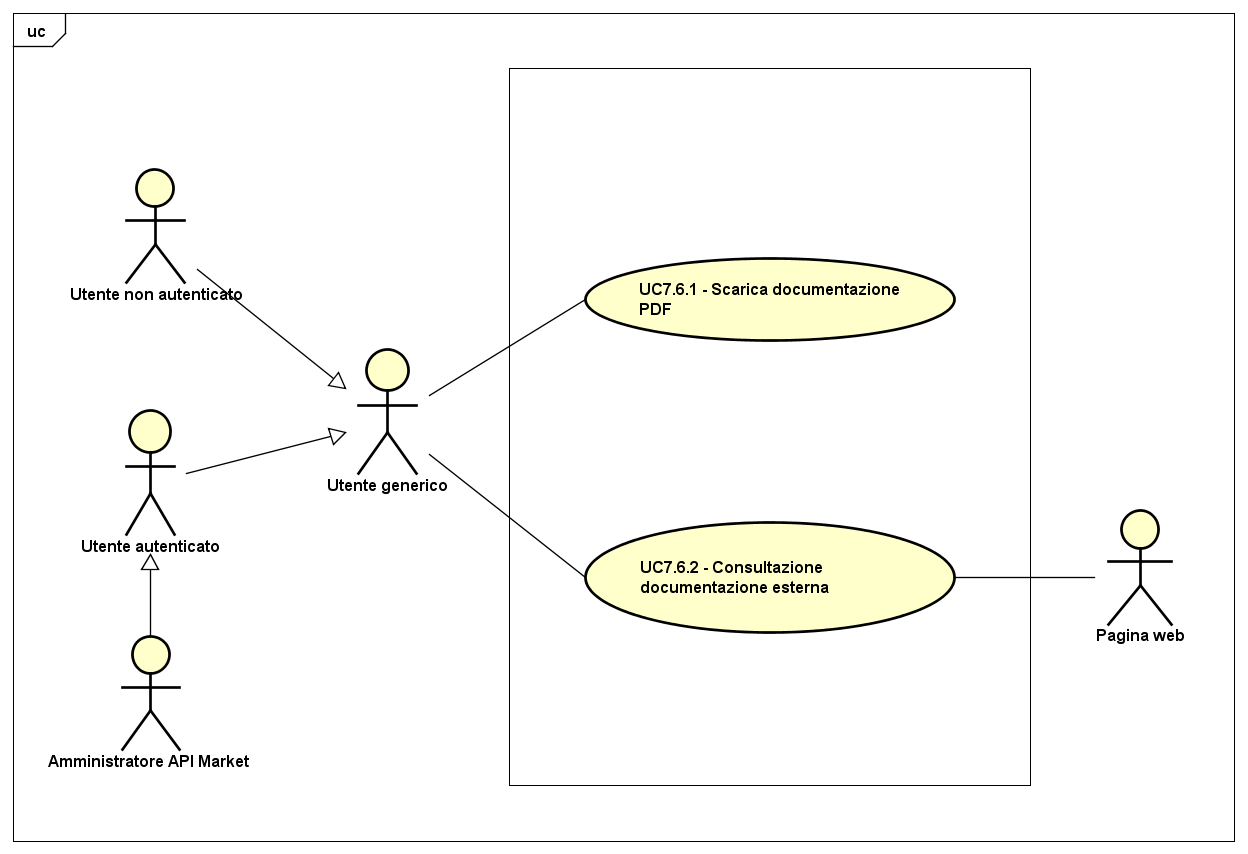
\includegraphics[scale=0.45]{UML/UC7_6.png}
	\caption{UC7.6: Visualizzazione API}
\end{figure}

\begin{minipage}{\linewidth}
	\begin{tabular}{ l | p{11cm}}
		\hline
		\rowcolor{Gray}
		\multicolumn{2}{c}{UC7.6 - Consultazione documentazione API} \\
		\hline
		\textbf{Attori} & Utente generico \\
		\textbf{Descrizione} & L'attore consulta la documentazione dell'API \\
		\textbf{Pre-Condizioni} & L'attore si trova nella schermata di visualizzazione API dell'API precedentemente selezionata \\
		\textbf{Post-Condizioni} & L'attore ha consultato la documentazione dell'API selezionata \\
		\textbf{Scenario Principale} & 
		\begin{enumerate*}[label=(\arabic*.),itemjoin={\newline}]
			\item L'attore può consultare la documentazione dell'API selezionata scaricando il file PDF fornito dall'autore (UC7.6.1)
			\item L'attore può consultare la documentazione dell'API selezionata tramite un link esterno fornita dall'autore (UC7.6.2)
		\end{enumerate*}\\
	\end{tabular}
\end{minipage}

\paragraph{Caso d'uso UC7.6.1: Scarica documentazione PDF}
\label{UC7_6_1}

\begin{minipage}{\linewidth}
	\begin{tabular}{ l | p{11cm}}
		\hline
		\rowcolor{Gray}
		\multicolumn{2}{c}{UC7.6.1 - Scarica documentazione PDF} \\
		\hline
		\textbf{Attori} & Utente generico \\
		\textbf{Descrizione} & L'attore scarica la documentazione dell'API in formato PDF tramite un link \\
		\textbf{Pre-Condizioni} & L'attore si trova nella schermata relativa alla consultazione della documentazione dell'API \\
		\textbf{Post-Condizioni} & L'attore ha scaricato la documentazione dell'API in formato PDF \\
		\textbf{Scenario Principale} & 
		\begin{enumerate*}[label=(\arabic*.),itemjoin={\newline}]
			\item L'attore può scaricare la documentazione dell'API in formato PDF
		\end{enumerate*}\\
	\end{tabular}
\end{minipage}

\paragraph{Caso d'uso UC7.6.2: Consultazione documentazione esterna}
\label{UC7_6_2}

\begin{minipage}{\linewidth}
	\begin{tabular}{ l | p{11cm}}
		\hline
		\rowcolor{Gray}
		\multicolumn{2}{c}{UC7.6.2 - Consultazione documentazione esterna} \\
		\hline
		\textbf{Attori} & Utente generico, Pagina web \\
		\textbf{Descrizione} & L'attore consulta la documentazione dell'API tramite un link esterno fornito dall'autore \\
		\textbf{Pre-Condizioni} & L'attore si trova nella schermata relativa alla consultazione della documentazione dell'API \\
		\textbf{Post-Condizioni} & L'attore ha aperto il link alla documentazione esterna dell'API ed è stato reindirizzato ad una pagina esterna specificata dall'autore dell'API \\
		\textbf{Scenario Principale} & 
		\begin{enumerate*}[label=(\arabic*.),itemjoin={\newline}]
			\item L'attore può consultare la documentazione esterna dell'API aprendo il link ad una pagina esterna specificata dall'autore dell'API
		\end{enumerate*}\\
	\end{tabular}
\end{minipage}

\newpage
\subsubsection{Caso d'uso UC7.7: Visualizzazione dati di utilizzo API}
\label{UC7_7}
\begin{figure}[ht]
	\centering
	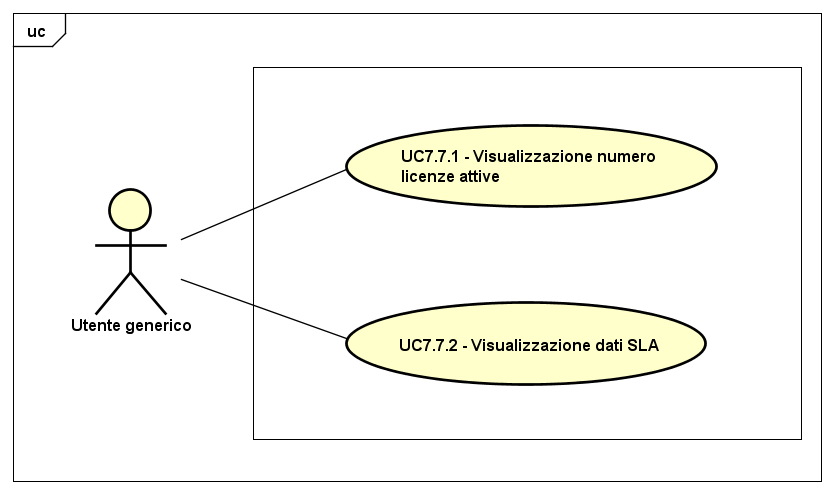
\includegraphics[scale=0.45]{UML/UC7_7.png}
	\caption{UC7.7: Visualizzazione API}
\end{figure}

\begin{minipage}{\linewidth}
	\begin{tabular}{ l | p{11cm}}
		\hline
		\rowcolor{Gray}
		\multicolumn{2}{c}{UC7.7 - Visualizzazione dati di utilizzo API} \\
		\hline
		\textbf{Attori} & Utente generico \\
		\textbf{Descrizione} & L'attore visualizza nella schermata relativa i dati di utilizzo dell'API \\
		\textbf{Pre-Condizioni} & L'attore si trova nella schermata di visualizzazione API dell'API precedentemente selezionata \\
		\textbf{Post-Condizioni} & L'attore ha visualizzato i dati di utilizzo dell'API selezionata \\
		\textbf{Scenario Principale} & 
		\begin{enumerate*}[label=(\arabic*.),itemjoin={\newline}]
			\item L'attore può visualizzare il numero di licenze attive per l'API selezionata (UC7.7.1)
			\item L'attore può visualizzare i dati di SLA dell'API selezionata (UC7.7.2)
		\end{enumerate*}\\
	\end{tabular}
\end{minipage}

\paragraph{Caso d'uso UC7.7.1: Visualizzazione numero licenze attive}
\label{UC7_7_1}

\begin{minipage}{\linewidth}
	\begin{tabular}{ l | p{11cm}}
		\hline
		\rowcolor{Gray}
		\multicolumn{2}{c}{UC7.7.1 - Visualizzazione numero licenze attive} \\
		\hline
		\textbf{Attori} & Utente generico \\
		\textbf{Descrizione} & L'attore visualizza il numero di licenze attive per l'API selezionata \\
		\textbf{Pre-Condizioni} & L'attore si trova nella schermata di visualizzazione dati di utilizzo API \\
		\textbf{Post-Condizioni} & L'attore ha visualizzato il numero di licenze attive per l'API selezionata \\
		\textbf{Scenario Principale} & 
		\begin{enumerate*}[label=(\arabic*.),itemjoin={\newline}]
			\item L'attore può visualizzare il numero di licenze attive per l'API selezionata
		\end{enumerate*}\\
	\end{tabular}
\end{minipage}

\paragraph{Caso d'uso UC7.7.2: Visualizzazione dati SLA}
\label{UC7_7_2}

\begin{minipage}{\linewidth}
	\begin{tabular}{ l | p{11cm}}
		\hline
		\rowcolor{Gray}
		\multicolumn{2}{c}{UC7.7.2 - Visualizzazione dati SLA} \\
		\hline
		\textbf{Attori} & Utente generico \\
		\textbf{Descrizione} & L'attore visualizza  all'API selezionata \\
		\textbf{Pre-Condizioni} & L'attore si trova nella schermata di visualizzazione dati di utilizzo API \\
		\textbf{Post-Condizioni} & L'attore ha visualizzato i dati di SLA dell'API selezionata \\
		\textbf{Scenario Principale} & 
		\begin{enumerate*}[label=(\arabic*.),itemjoin={\newline}]
			\item L'attore può visualizzare i dati di SLA dell'API selezionata
		\end{enumerate*}\\
	\end{tabular}
\end{minipage}

\subsubsection{Caso d'uso UC7.8: Visualizzazione prezzo API}
\label{UC7_8}

\begin{minipage}{\linewidth}
	\begin{tabular}{ l | p{11cm}}
		\hline
		\rowcolor{Gray}
		\multicolumn{2}{c}{UC7.8 - Visualizzazione prezzo API} \\
		\hline
		\textbf{Attori} & Utente generico \\
		\textbf{Descrizione} & L'attore visualizza nella schermata relativa il prezzo dell'API \\
		\textbf{Pre-Condizioni} & L'attore si trova nella schermata di visualizzazione API dell'API precedentemente selezonata \\
		\textbf{Post-Condizioni} & L'attore ha visualizzato il prezzo dell'API selezionata \\
		\textbf{Scenario Principale} & 
		\begin{enumerate*}[label=(\arabic*.),itemjoin={\newline}]
			\item L'attore può visualizzare il prezzo dell'API (secondo la policy stabilita dall'autore)
		\end{enumerate*}\\
	\end{tabular}
\end{minipage}

\subsubsection{Caso d'uso UC7.9: Visualizzazione data ultima modifica API}
\label{UC7_9}

\begin{minipage}{\linewidth}
	\begin{tabular}{ l | p{11cm}}
		\hline
		\rowcolor{Gray}
		\multicolumn{2}{c}{UC7.9 - Visualizzazione data ultima modifica API} \\
		\hline
		\textbf{Attori} & Utente autenticato, Amministratore API Market \\
		\textbf{Descrizione} & L'attore visualizza nella schermata relativa la data dell'ultima modifica effettuata sull'API \\
		\textbf{Pre-Condizioni} & L'attore ha selezionato una API, ne possiede la licenza attiva e si trova nella schermata di visualizzazione API \\
		\textbf{Post-Condizioni} & L'attore ha visualizzato nella schermata relativa la data dell'ultima modifica effettuata sull'API selezionata \\
		\textbf{Scenario Principale} & 
		\begin{enumerate*}[label=(\arabic*.),itemjoin={\newline}]
			\item L'attore può visualizzare nella schermata relativa la data dell'ultima modifica effettuata sull'API selezionata
		\end{enumerate*}\\
	\end{tabular}
\end{minipage}

\subsubsection{Caso d'uso UC7.10: Visualizzazione versione API}
\label{UC7_10}

\begin{minipage}{\linewidth}
	\begin{tabular}{ l | p{11cm}}
		\hline
		\rowcolor{Gray}
		\multicolumn{2}{c}{UC7.10 - Visualizzazione versione API} \\
		\hline
		\textbf{Attori} & Utente generico \\
		\textbf{Descrizione} & L'attore visualizza nella schermata relativa la versione dell'API \\
		\textbf{Pre-Condizioni} & L'attore si trova nella schermata di visualizzazione API dell'API precedentemente selezonata \\
		\textbf{Post-Condizioni} & L'attore ha visualizzato la versione dell'API selezionata \\
		\textbf{Scenario Principale} & 
		\begin{enumerate*}[label=(\arabic*.),itemjoin={\newline}]
			\item L'attore può visualizzare la versione dell'API
		\end{enumerate*}\\
	\end{tabular}
\end{minipage}

\subsubsection{Caso d'uso UC7.11: Visualizzazione logo API}
\label{UC7_11}

\begin{minipage}{\linewidth}
	\begin{tabular}{ l | p{11cm}}
		\hline
		\rowcolor{Gray}
		\multicolumn{2}{c}{UC7.11 - Visualizzazione logo API} \\
		\hline
		\textbf{Attori} & Utente generico \\
		\textbf{Descrizione} & L'attore visualizza nella schermata relativa il logo dell'API \\
		\textbf{Pre-Condizioni} & L'attore si trova nella schermata di visualizzazione API dell'API precedentemente selezonata \\
		\textbf{Post-Condizioni} & L'attore ha visualizzato il logo dell'API selezionata \\
		\textbf{Scenario Principale} & 
		\begin{enumerate*}[label=(\arabic*.),itemjoin={\newline}]
			\item L'attore può visualizzare il logo dell'API
		\end{enumerate*}\\
	\end{tabular}
\end{minipage}

\subsubsection{Caso d'uso UC7.12: Visualizzazione policy vendita API}
\label{UC7_12}

\begin{minipage}{\linewidth}
	\begin{tabular}{ l | p{11cm}}
		\hline
		\rowcolor{Gray}
		\multicolumn{2}{c}{UC7.12 - Visualizzazione policy vendita API} \\
		\hline
		\textbf{Attori} & Utente generico \\
		\textbf{Descrizione} & L'attore visualizza nella schermata relativa la policy di vendita dell'API \\
		\textbf{Pre-Condizioni} & L'attore si trova nella schermata di visualizzazione API dell'API precedentemente selezonata \\
		\textbf{Post-Condizioni} & L'attore ha visualizzato la policy di vendita dell'API selezionata \\
		\textbf{Scenario Principale} & 
		\begin{enumerate*}[label=(\arabic*.),itemjoin={\newline}]
			\item L'attore può visualizzare la policy di vendita dell'API
		\end{enumerate*}\\
	\end{tabular}
\end{minipage}

\subsubsection{Caso d'uso UC7.13: Visualizzazione link acquisto API}
\label{UC7_13}

\begin{minipage}{\linewidth}
	\begin{tabular}{ l | p{11cm}}
		\hline
		\rowcolor{Gray}
		\multicolumn{2}{c}{UC7.13 - Visualizzazione link acquisto API} \\
		\hline
		\textbf{Attori} & Utente generico \\
		\textbf{Descrizione} & L'attore visualizza nella schermata relativa il link alla pagina d'acquisto dell'API \\
		\textbf{Pre-Condizioni} & L'attore si trova nella schermata di visualizzazione API dell'API precedentemente selezonata \\
		\textbf{Post-Condizioni} & L'attore ha visualizzato il link alla pagina d'acquisto dell'API selezionata \\
		\textbf{Scenario Principale} & 
		\begin{enumerate*}[label=(\arabic*.),itemjoin={\newline}]
			\item L'attore può visualizzare il link alla pagina d'acquisto dell'API
		\end{enumerate*}\\
	\end{tabular}
\end{minipage}